%!TEX root = ../PhDthesis.tex
\chapter{Appendix}

\section{HoloViews: Building Complex Visualizations Easily} \label{SciPyPaper}

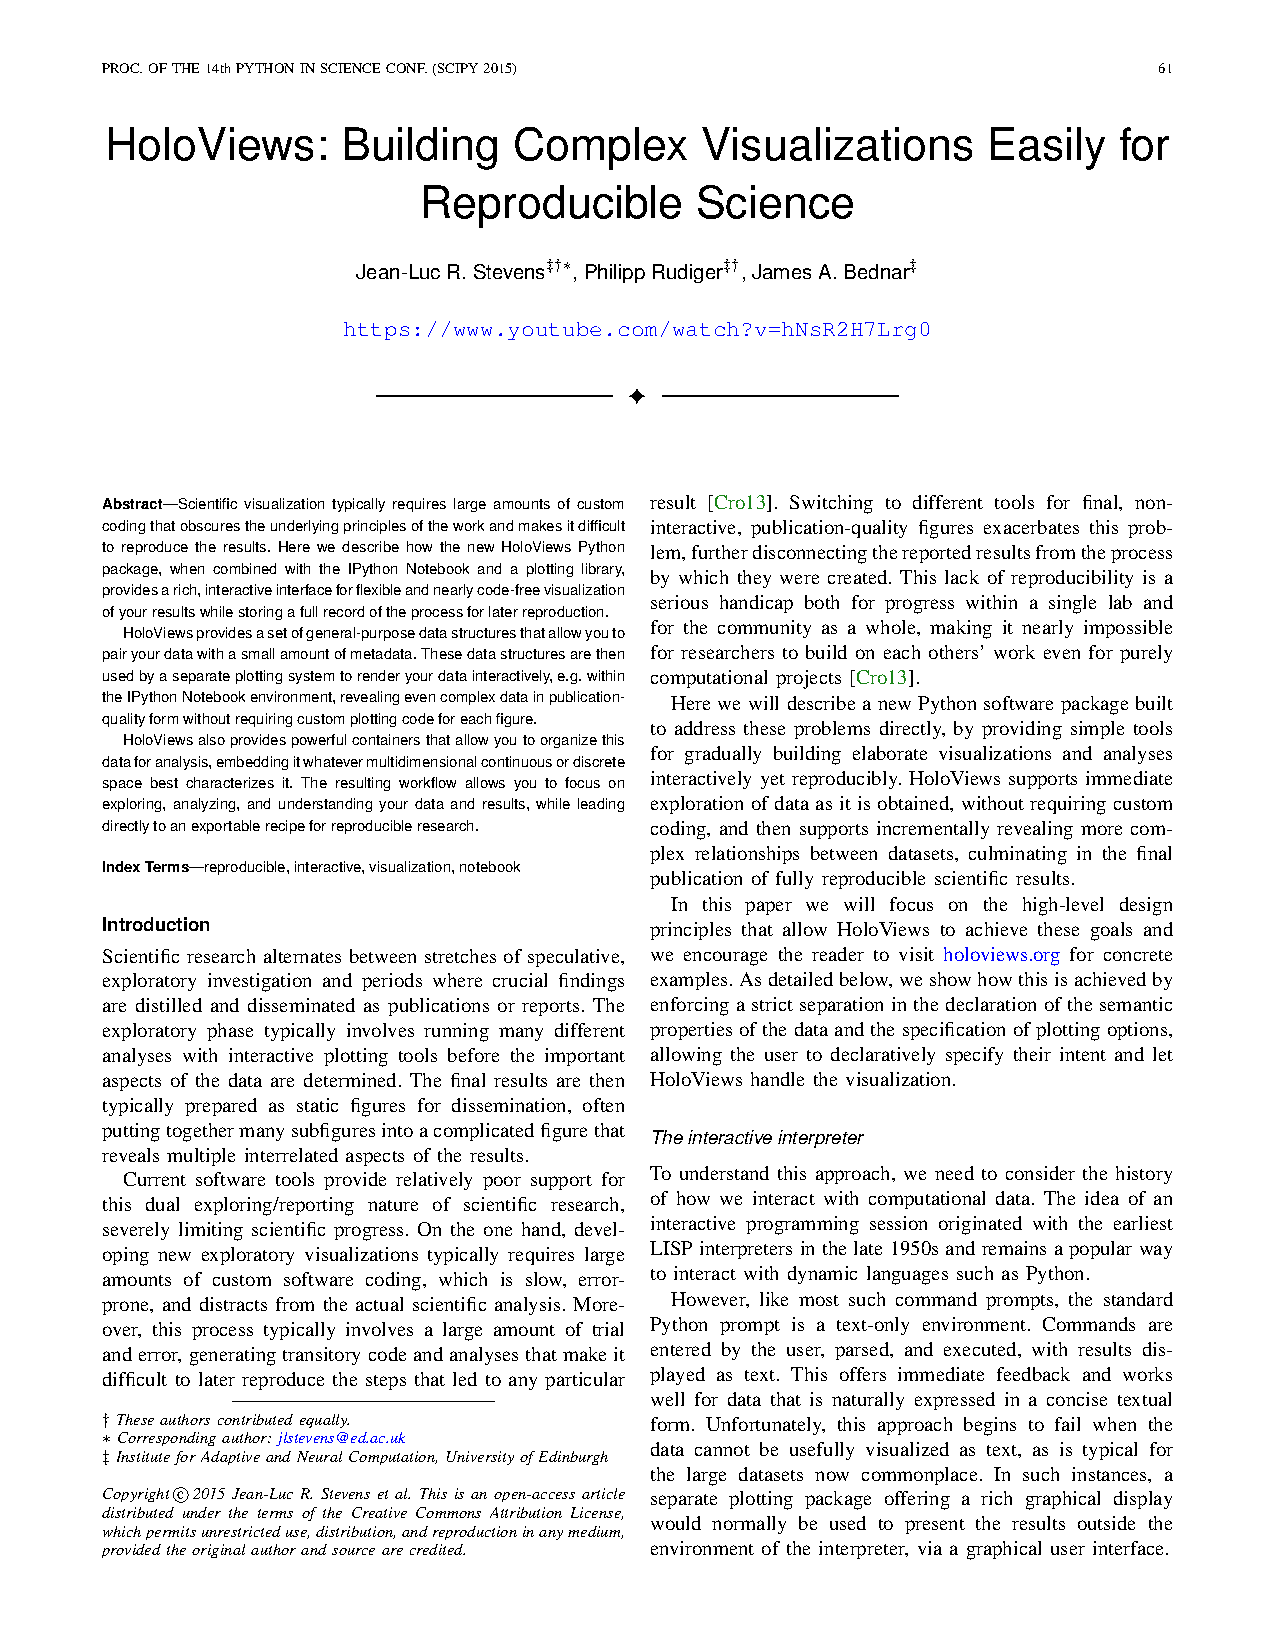
\includepdf[pages=-]{./SciPyPaper.pdf}

\section{Model Parameters} \label{Appendix:Parameters}

{\renewcommand{\arraystretch}{0.7}
\begin{tabular}{ l l l }
  \hline
	Symbol & Description & Value \\ \hline
	\ & \textbf{RGC/LGN}  & \  \\
	$\gamma_A$ & Strength of the retinogeniculate projection & 14 \\
	$\gamma_L$ & Strength of the lateral gain control & 0.6 \\
	$\sigma_C$ & Size of the center component & 0.2 \\
	$\sigma_S$ & Size of the surround component & 0.3 \\
	$\sigma_L$ & Size of the lateral gain control component & 0.25 \\
	$c$ & Constant offset of the lateral gain control function & 0.11 \\
	$\kappa_A$ & Cut-off radius of the afferent projection & 0.3 \\
	$\kappa_L$ & Cut-off radius of the lateral gain control projection & 0.5 \\
	\ & \textbf{SCAL V1}  & \  \\
	$\gamma_A$ & Strength of the geniculocortical projections & 2.4 \\
	$\gamma_E$ & Strength of the local excitatory projection & 1.6 \\
	$\gamma_I$ & Strength of the divisive inhibitory projection & 1.8 \\
	$\gamma_{LE}$ & Strength of lateral excitatory projection & 0 \\
	$\sigma_E$ & Size of local excitatory projection & 0.06 \\
	$\sigma_I$ & Size of inhibitory projection & 0.12 \\
	$\sigma_L$ & Size of lateral excitatory projection & 1.25 \\
	$\kappa_A$ & Cut-off radius of afferent projection & 0.5 \\
	$\kappa_E$ & Cut-off radius of local excitatory projection & 0.14 \\
	$\kappa_I$ & Cut-off radius of inhibitory projection & 0.18 \\
	$\kappa_L$ & Cut-off radius of lateral excitatory projection & 1.25 \\
	$\lambda_A$ & Learning-rate of the afferent projections & 0.1 \\
	$\lambda_E$ & Learning-rate of the local excitatory projection & 0 \\
	$\lambda_I$ & Learning-rate of the inhibitory projection & 0.3 \\
	$\lambda_L$ & Learning-rate of the lateral excitatory projection & 1 \\
	$\tau_L$ & Time constant of lateral projection hysteresis function & 0.2 \\
	\ & \textbf{SEPI V1 Excitatory} (Only changed)  & \  \\
	$\gamma_A$ & Strength of the afferent projection & 3 \\
	$\gamma_E$ & Strength of local excitatory projection & 2.5 \\
	$\gamma_L$ & Strength of lateral excitatory projection & 0 \\
	$\lambda_A$ & Learning-rate of the afferent projections & 0.25 \\
	$\lambda_E$ & Learning-rate of the local excitatory projection & 0 \\
	$\lambda_L$ & Learning-rate of the lateral excitatory projection & 1 \\
	\ & \textbf{SEPI V1 Parvalbumin} (Only changed)  & \  \\
	$\gamma_P$ & Strength of the divisive inhibitory projection & 2.5 \\
	$\gamma_{RP}$ & Strength of the recurrent divisive inhibitory projection & 0.8 \\
	$\lambda_P$ & Learning rate of lateral inhibitory projection & 0.25 \\
	\ & \textbf{LESPI V1 Excitatory} (Only changed) & \  \\
	$\gamma_L$ & Strength of lateral excitatory projection & 3 \\
	$\gamma_{ES}$ & Strength of local excitatory projection to Sst cells & 0.6 \\
	$\gamma_{LS}$ & Strength of lateral excitatory projection to Sst cells & 6 \\
	$\lambda_{LS}$ & Learning rate of lateral excitatory projection to Sst cells & 5 \\
	$\beta_{LS}$ & Exponent of the lateral excitatory projection to Sst cells & 3 \\
	\ & \textbf{LESPI V1 Somatostatin} & \  \\
	$\gamma_S$ & Strength of Sst inhibition projection & -1 \\
	$\tau_S$ & Time constant of Sst neuron hysteresis function & 0.2 \\
	$\lambda_S$ & Learning rate of Sst inhibition projection & 0.1 \\
\end{tabular}}

